\section{Methods}
\label{sec:methods}

\subsection{Optimizer}
The choice of optimizer is critical for the convergence and performance of deep learning models. We experimented with several optimizers, including Stochastic Gradient Descent (SGD), Adam, and RMSprop. Our final choice was based on empirical performance and convergence speed, aligning with findings in Kingma and Ba (2014) \cite{kingma2014adam}.

\subsection{Lp Regularization}
To prevent overfitting, we incorporated Lp regularization techniques, including L2 (Ridge) and L1 (Lasso) regularization. These techniques add a penalty to the loss function, proportional to the magnitude of the coefficients, thus encouraging the model to maintain simpler and more generalizable parameters \cite{ng2004feature}.

\subsection{Cross-Validation}
We utilized k-fold cross-validation to rigorously evaluate the performance of our model. This method involves partitioning the dataset into k subsets, training the model on k-1 subsets, and validating it on the remaining subset. This process is repeated k times, with each subset serving as the validation set once. Cross-validation provides a comprehensive assessment of the model’s generalizability \cite{kohavi1995study}.

\subsection{Data Augmentation}
Data augmentation is a widely used technique in machine learning and deep learning to increase the diversity and quantity of training data, ultimately improving the generalization capability of models. New training samples are generated by applying various transformations (such as rotation, flipping, scaling, etc.) to the original data, thus increasing the diversity and quantity of the dataset. The model can then learn more feature representations, leading to improved performance on unseen data \cite{shorten2019survey}.

\subsection{Generating Extra Dataset}
To augment our training data, we tried to utilize the Deep Convolutional Generative Adversarial Network (DCGAN) and the Diffusion Model. These techniques can generates synthetic data that resembles the real dataset, thereby increasing the diversity and quantity of training examples. This approach is particularly beneficial when the available labeled data is limited \cite{radford2015unsupervised}.

\subsection{Pretrained Model}
For our initial model weights, we employed a pretrained Vision Transformer. Pretrained models provide a significant advantage by leveraging features learned from large-scale datasets, thereby improving the performance and convergence speed on our specific task \cite{dosovitskiy2020image}.

\subsection{Hyperparameter Tuning}
Hyperparameter tuning was performed using a grid search approach. Key hyperparameters tuned included the learning rate, batch size, and regularization coefficients. The optimal hyperparameters were selected based on validation performance \cite{bergstra2012random}.

\subsection{Ensemble Learning}
Besides the methods of ResNet and the ViT, we also tried the VLM (Visual-Linguistic Model) to improve the performance of the classifier. So we need to use the Method of Ensemble Learning, utilizing multiple methods as base learners and combining results of these methods, for improving overall predictive performance and robustness of the classifier \cite{zhou2012ensemble}.

\subsection{Attention Mechanism and Visualization}
To enhance our model's ability to focus on discriminative regions of the image, which is crucial for fine-grained visual classification, we incorporated an attention mechanism within our Vision Transformer architecture. Attention mechanisms allow the model to allocate more 'attention' or importance to those parts of the image that are more relevant for distinguishing between highly similar subcategories \cite{vaswani2017attention}.

To visualize how our model focuses on these critical regions, we employ Class Activation Mapping (CAM) techniques. CAM provides a heat map overlay on the input image, indicating the regions most influential for the model's decision \cite{zhou2016learning}.

\begin{figure}[h]
    \centering
    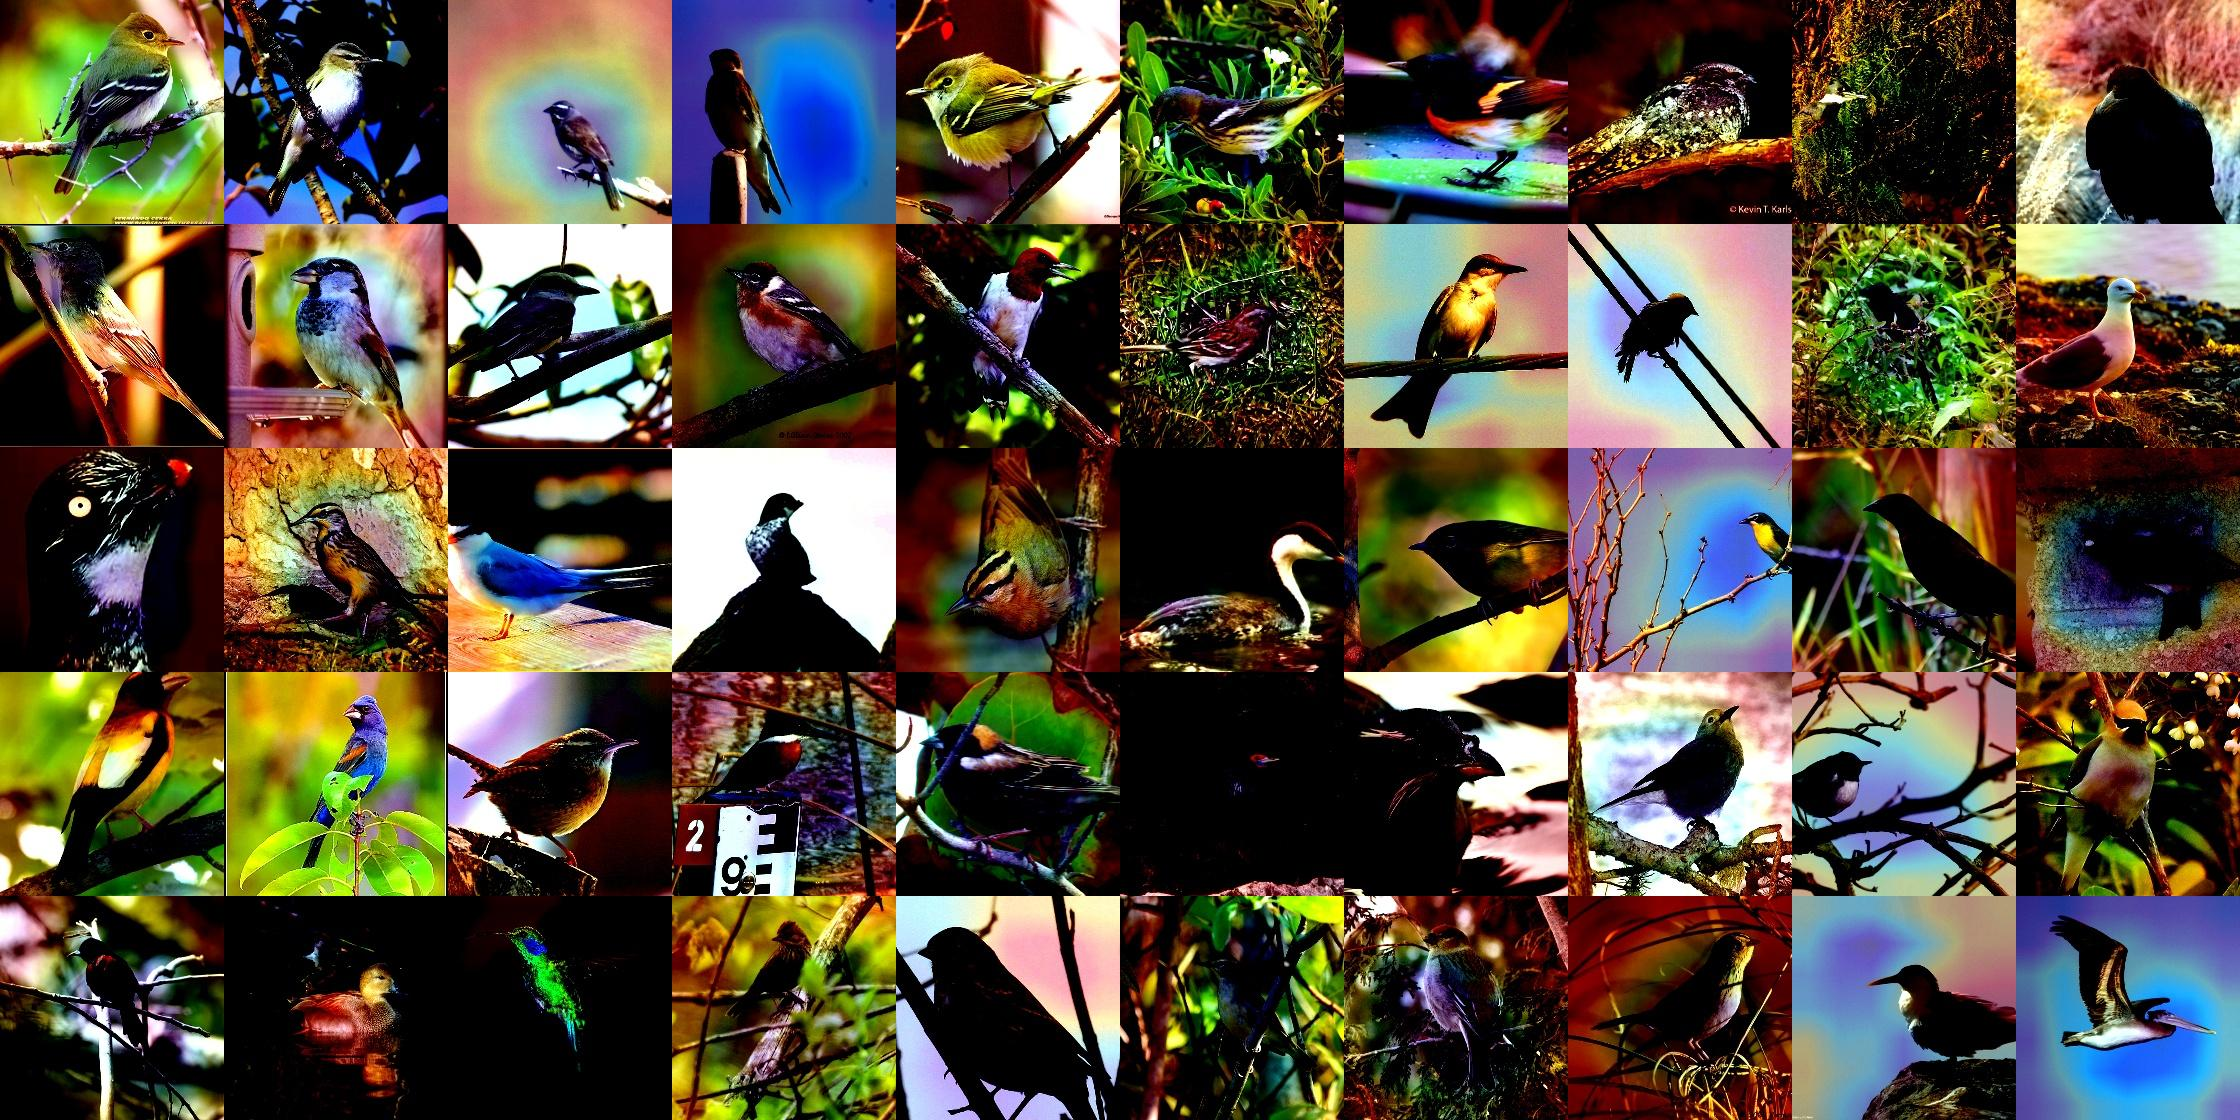
\includegraphics[width=\linewidth]{res/output_grid.jpg}
    \caption{Visualization of the attention mechanism using CAM, highlighting areas of importance that contribute to model decisions.}
    \label{fig:cam_attention}
\end{figure}
